\section{需求分析概述}

\subsection{需求分析的根本任务}

\begin{figure}[H]
	\centering
    \vspace{-1em}
	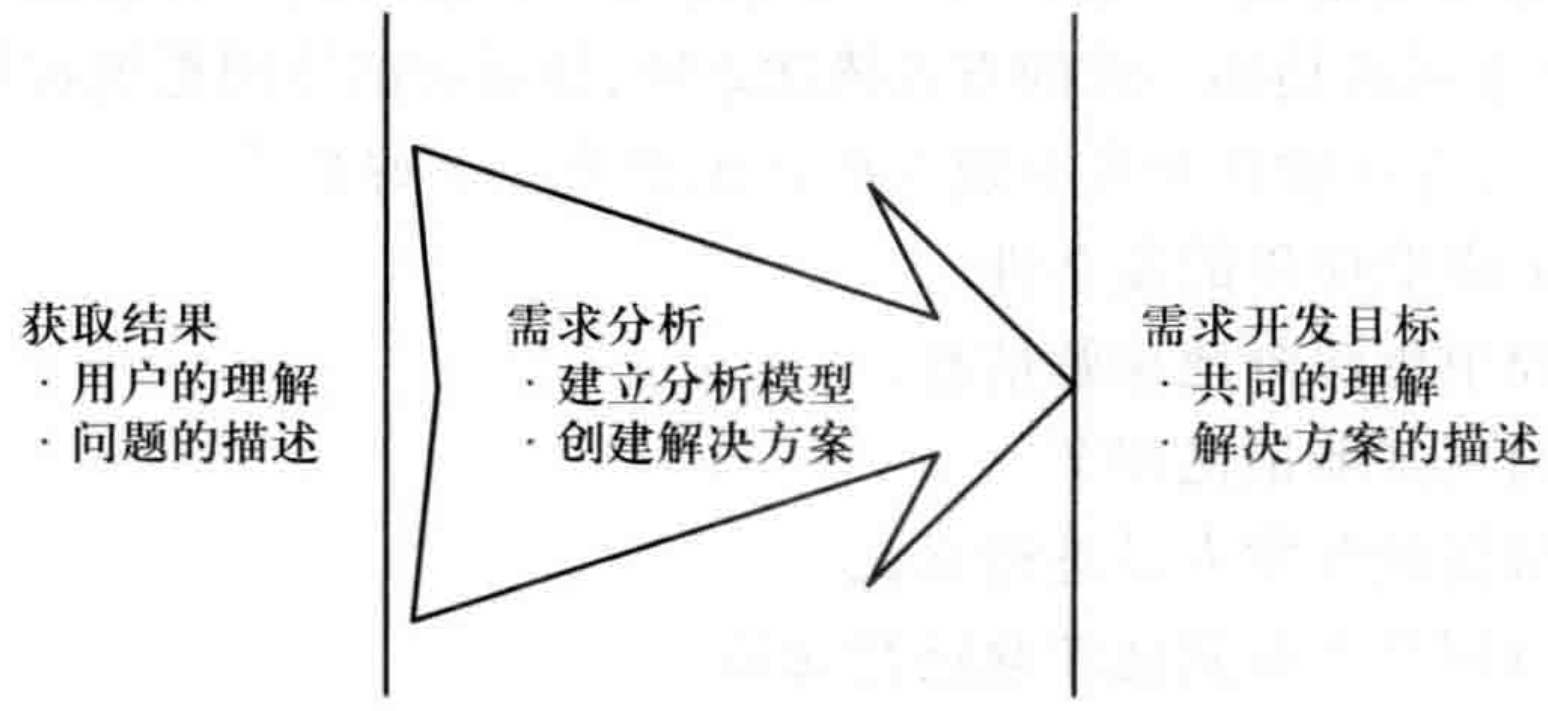
\includegraphics[width=0.55\textwidth]{img/需求分析的任务.png}
    \vspace{-1em}
\end{figure}

需求分析的根本任务有如下两条:
\begin{itemize}
    \item 建立分析模型
    \begin{itemize}
        \item 将复杂的系统分解成为简单的部分以及它们之间的联系,确定本质特征
        \item 和用户达成对信息内容的共同理解
        \item 分析的活动主要包括识别、定义和结构化,它的目的是获取某个可以转换为知识的事物的信息
    \end{itemize}
    \item 创建解决方案
    \begin{itemize}
        \item 将一个问题分解成独立的、更简单和易于管理的子问题来帮助寻找解决方案
        \item 创建解决方案的过程是创造性的
        \item 帮助开发者建立问题的定义,并确定被定义的事物之间的逻辑关系
        \begin{itemize}
            \item 这些逻辑关系可以形成信息的推理,进而可以被用来验证解决方案的正确性
        \end{itemize}
    \end{itemize}
\end{itemize}

\subsubsection{建立分析模型}

\paragraph{模型}~{} \par
“模型是对事物的抽象,帮助人们在创建一个事物之前可以有更好的理解” 

集中关注问题的计算特性(数据、功能、规则等等) 

“它是对系统进行思考和推理的一种方式。建模的目标是建立系统的一个表示,这个表示以精确一致的方式描述系统,使得系统的使用更加容易” 

建模方法
\begin{itemize}
    \item 抽象(Abstraction)
    \begin{itemize}
        \item 一方面要求人们只关注重要的信息,忽略次要的内容:通过强调本质的特征,就减少了问题的复杂性
        \item 另一方面也要求人们将认知保留在适当的层次,屏蔽更深层次的细节:在问题的各元素之间推断出更广泛和更普遍的关系,帮助人们寻找解决方案
    \end{itemize}
    \item 分解(Decomposition/Partitioning)
    \begin{itemize}
        \item “分而治之”:将单个复杂和难以理解的问题分解成多个相对更容易的子问题,并掌握各子问题之间的联系
        \item 分解的方案往往还能提供问题的解决思路
    \end{itemize}
    \item 投影(Projection)
    \begin{itemize}
        \item 多视点方法
    \end{itemize}
\end{itemize}

\paragraph{两个世界与三种模型}~{} \par
\textbf{计算世界与计算模型} \par
基于软件构建单位及其之间的关系建立的模型是软件工程中非常常用的一种模型形式,用来说明软件逻辑上的构建方式和实现方式。这种模型使用的组元及其关系都是软件的元素,所以它是来自于软件(计算世界)的模型,称为计算模型。

基于计算科学建立的,具有形式化的特征
\begin{itemize}
    \item 信息的描述具有明确化、准确化和确定化的特征
\end{itemize}

需求分析阶段不适宜建立形式化的计算模型
\vspace{-0.8em}
\begin{multicols}{2}
    \begin{itemize}
        \item 重点是问题,缺乏和软件实现相关的技术细节
        \item 用户无法理解
    \end{itemize}
\end{multicols}
\vspace{-1em}

\begin{figure}[H]
	\centering
    \vspace{-0.5em}
	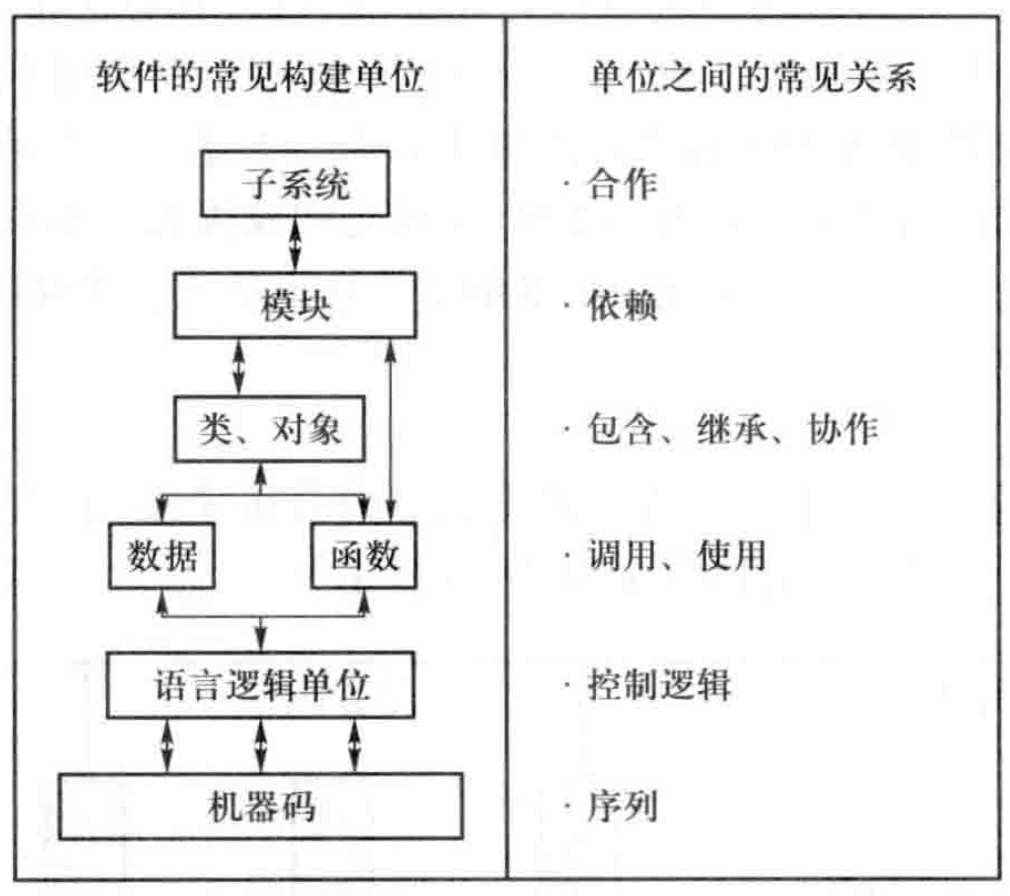
\includegraphics[width=0.53\textwidth]{img/软件的常见构建单位及其关系.png}
    \caption*{软件的常见构建单位及其关系}
    \vspace{-1em}
\end{figure}


\textbf{问题世界与业务模型} \par
业务模型使用问题域中的重要概念作为模型的组元,使用概念之间的业务联系作为组元之间的关系

使用了业务描述的方式,具有非形式化特征
\begin{itemize}
    \item 业务模型元素(即业务概念和业务联系)的选取和定义上具有不准确、不确定和模糊化
    \item 可以抽取出需求信息中最重要和最本质的内容
    \item 可以达成用户和开发者的共同理解
\end{itemize}

非形式化特征使得它不适合于进行需求建模
\begin{itemize}
    \item 不足以用于描述一个有效的软件解决方案:不准确、不确定和模糊化
\end{itemize}

\textbf{软件分析模型} \par
软件分析模型是介于计算模型和业务模型二者之间的模型形式,使用了计算模型的组元形式,在组元的表现上采用了业务模型的表现方式

\begin{figure}[H]
	\centering
    \vspace{-0.5em}
	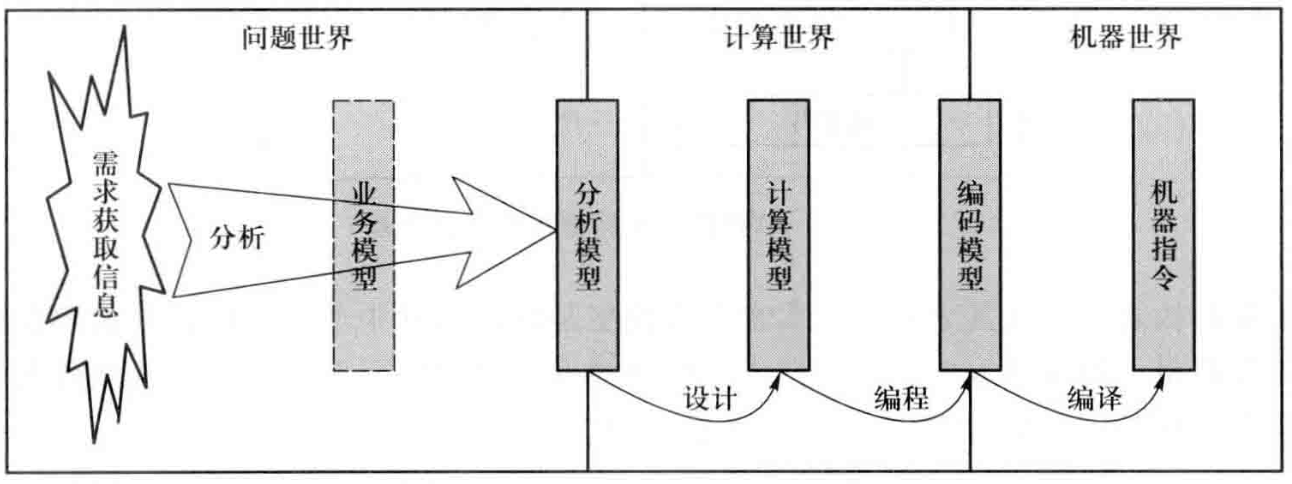
\includegraphics[width=0.75\textwidth]{img/软件分析模型.png}
    \caption*{软件分析模型}
    \vspace{-1em}
\end{figure}

软件分析模型是半形式化的,不再像计算模型那么严谨,不再具有形式化的特征,由于需求分析的半形式化特征还使得它可以比业务模型更严格

\textbf{三种模型的区别示例} \par
\begin{figure}[H]
	\centering
    \vspace{-0.5em}
	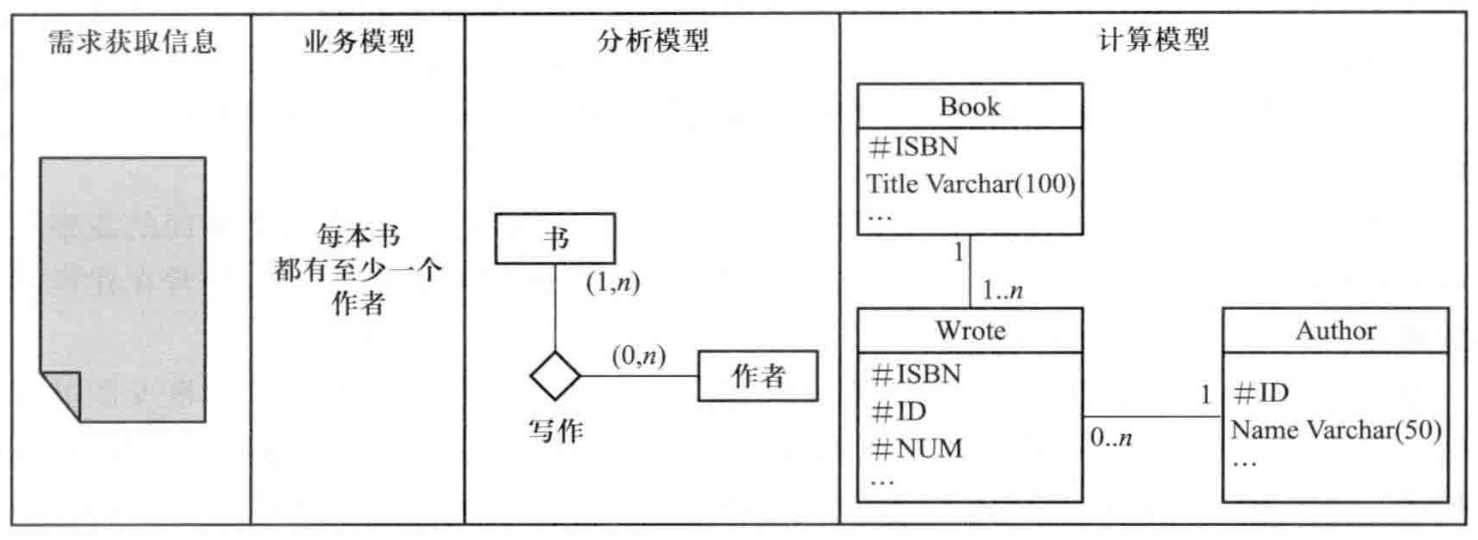
\includegraphics[width=0.75\textwidth]{img/3种模型的区别示例.png}
    \vspace{-1em}
\end{figure}

\paragraph{需求建模}~{} \par
需求建模通常的做法是:
\begin{itemize}
    \item 先依据获取的问题域信息建立初步的模型
    \item 然后分析用户需求,对模型进行调整,得到一个中间形式的模型形式
    \item 最后,对调整后的模型进行逻辑推理和验证,如果符合预期的期望,那么它就是最终的解决方案模型
\end{itemize}

\begin{figure}[H]
	\centering
    \vspace{-0.5em}
	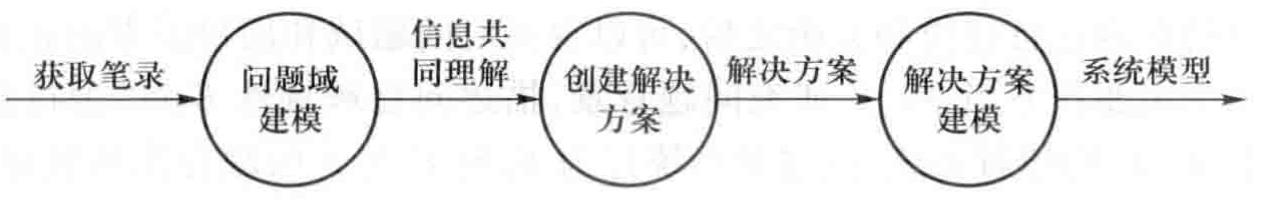
\includegraphics[width=0.7\textwidth]{img/需求建模过程.png}
    \caption*{需求建模过程}
    \vspace{-1em}
\end{figure}


\subsubsection{建立解决方案}
\begin{figure}[H]
	\setcounter{subfigure}{0}
	\centering
	\vspace{-1em}	
	\subfloat{
		\begin{minipage}[c]{0.48\linewidth}
		\centering
		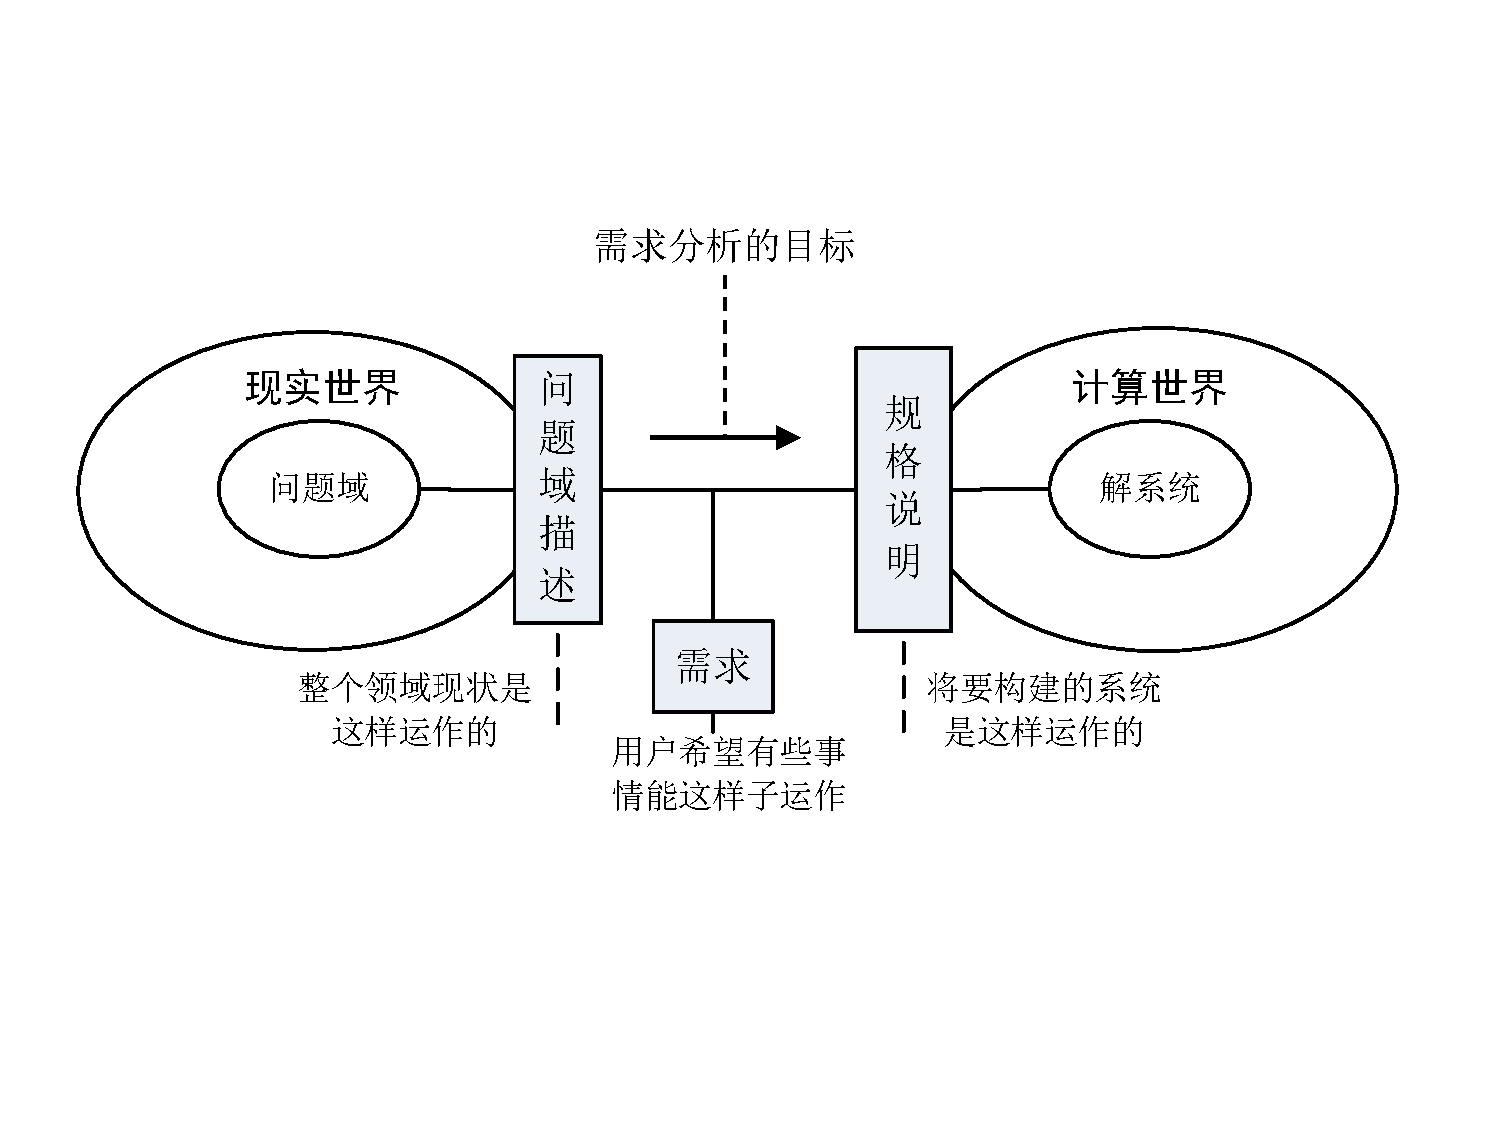
\includegraphics[width=\linewidth]{img/建立解决方案.pdf}
		\end{minipage}
	}
	\subfloat{
		\begin{minipage}[c]{0.49\linewidth}
		\centering
		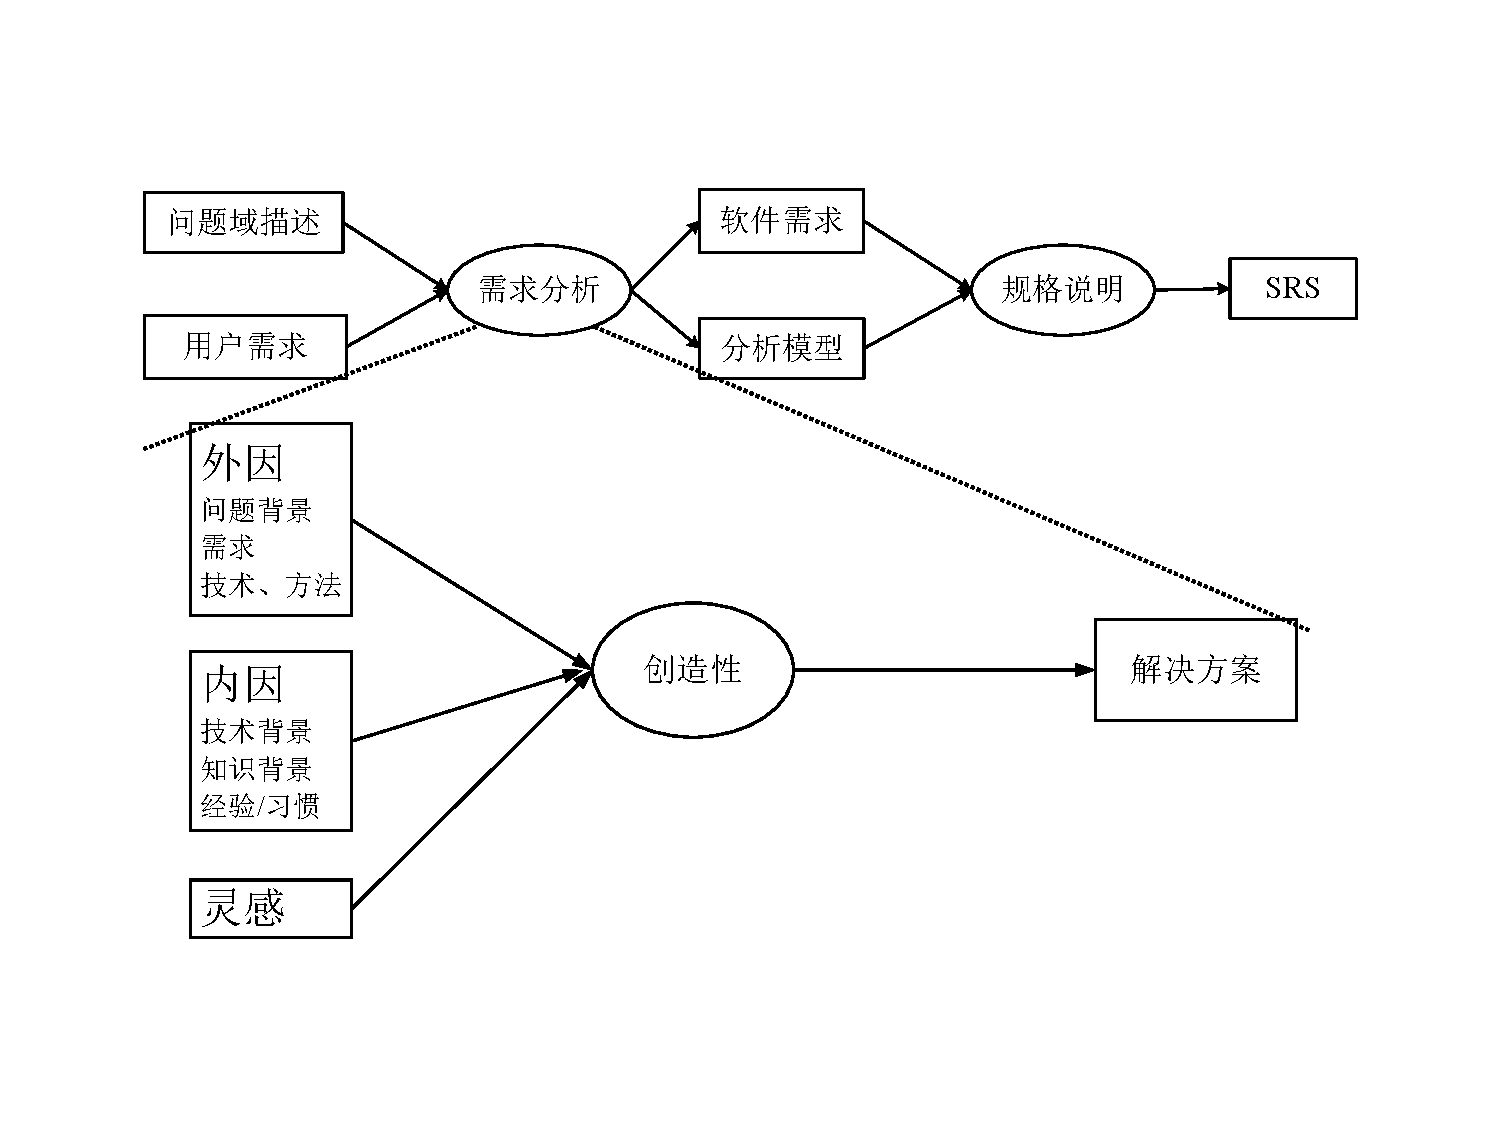
\includegraphics[width=\linewidth]{img/建立解决方案的过程.pdf}
		\end{minipage}
	}
	\centering
	\vspace{-1em}
\end{figure}

\subsection{需求分析方法}
\begin{figure}[H]
	\centering
    \vspace{-0.5em}
	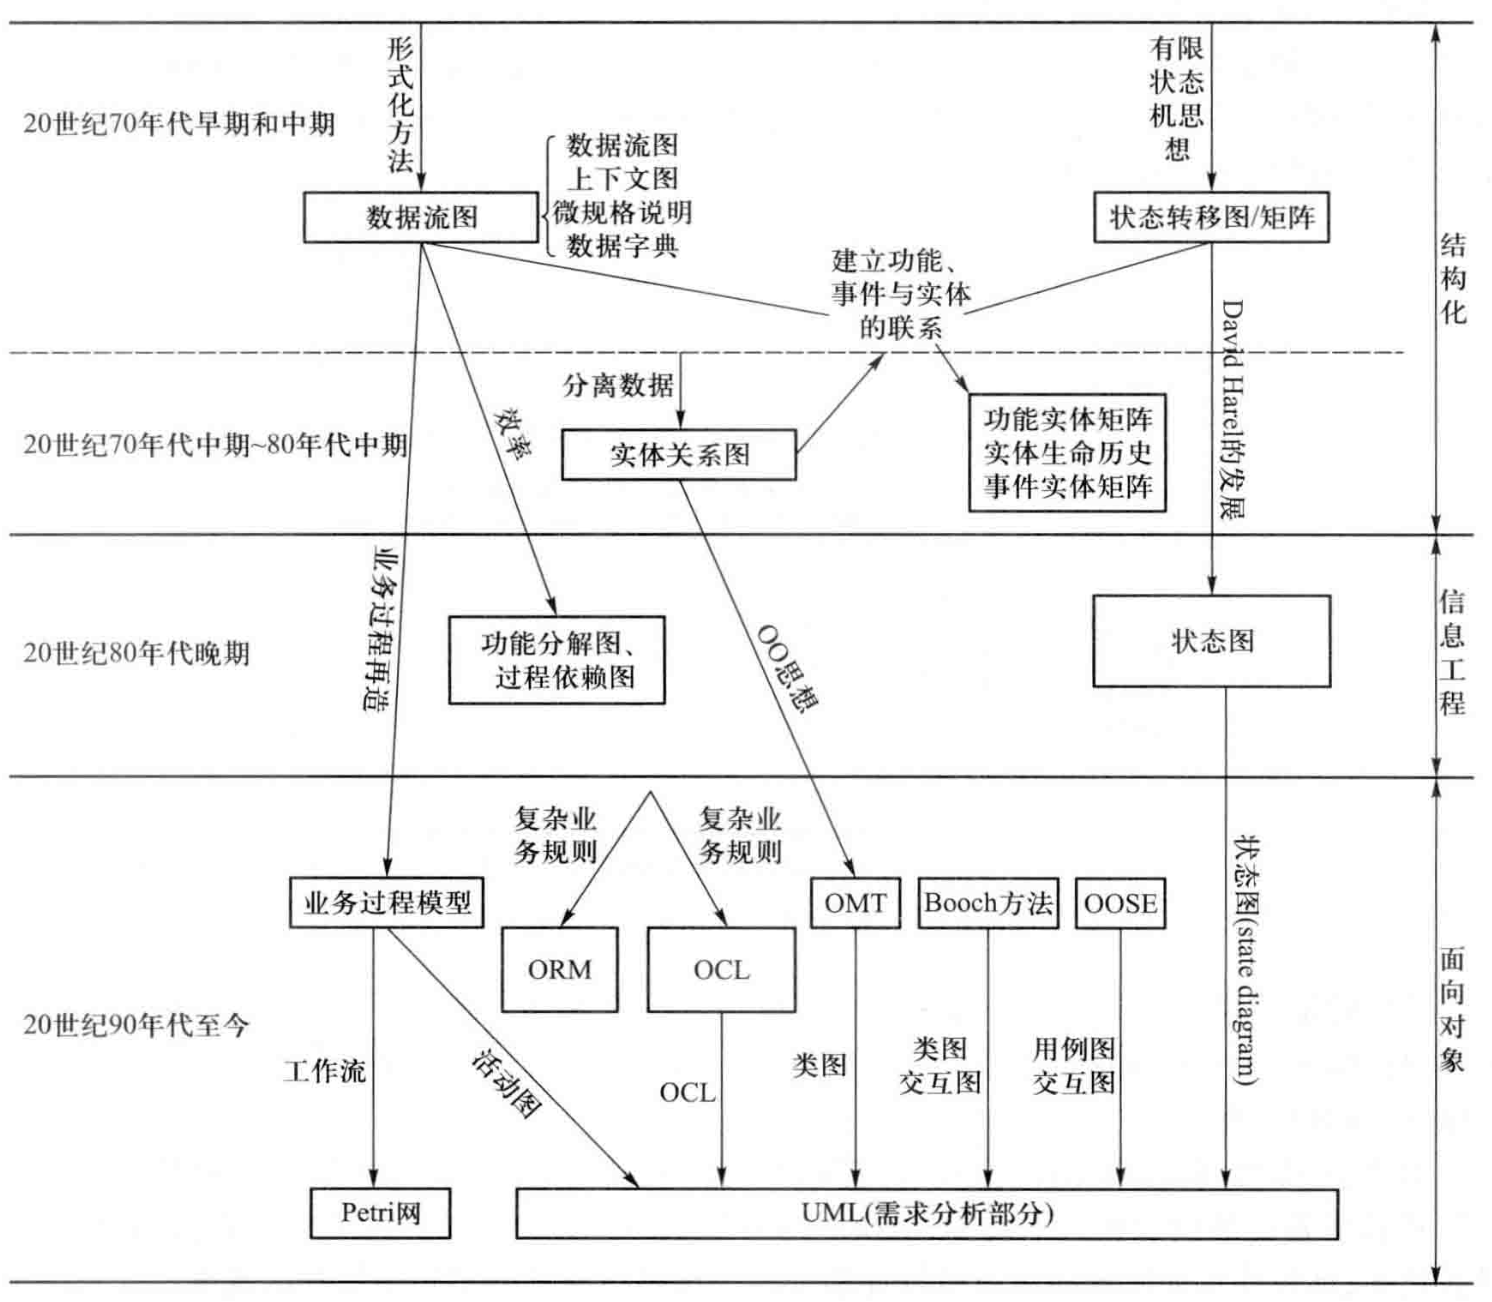
\includegraphics[width=0.9\textwidth]{img/常见需求分析技术的发展历程.png}
    \caption*{常见需求分析技术的发展历程}
    \vspace{-1em}
\end{figure}

\begin{figure}[H]
	\setcounter{subfigure}{0}
	\centering
	\vspace{-1em}	
	\subfloat{
		\begin{minipage}[c]{0.56\linewidth}
		\centering
		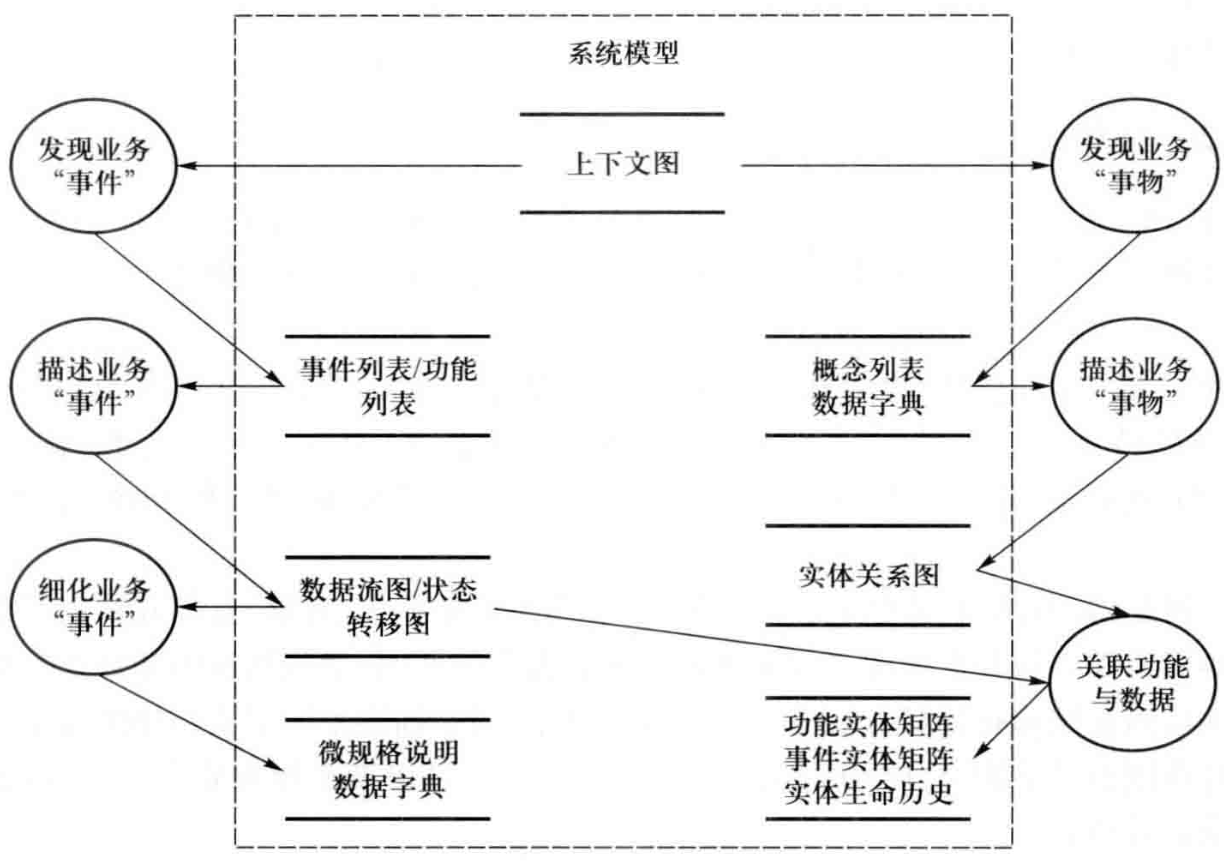
\includegraphics[width=\linewidth]{img/结构化分析的典型过程.png}
        \caption*{结构化分析的典型过程}
		\end{minipage}
	}
	\subfloat{
		\begin{minipage}[c]{0.37\linewidth}
		\centering
		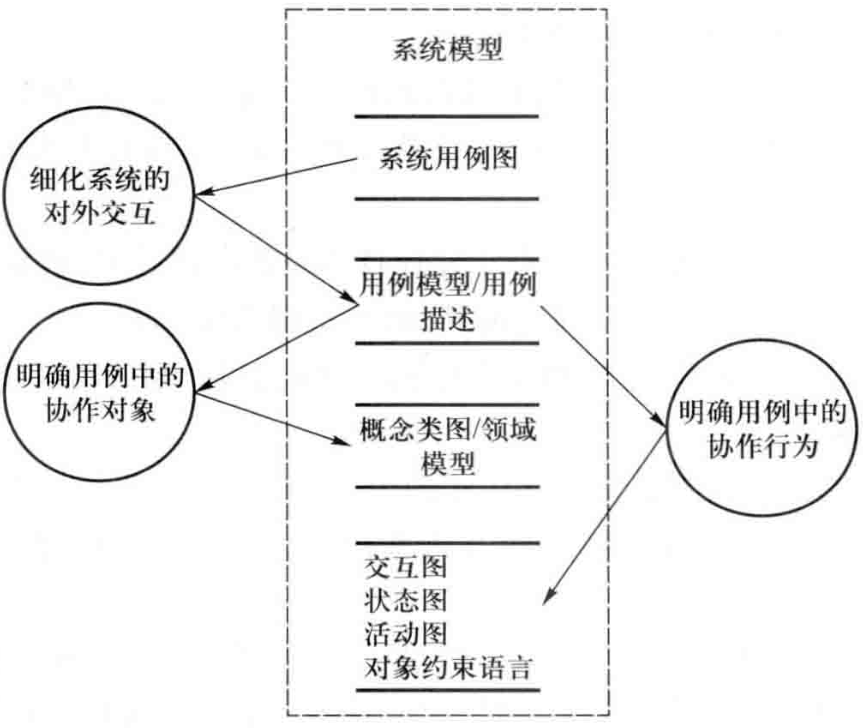
\includegraphics[width=\linewidth]{img/面向对象分析的典型过程.png}
        \caption*{面向对象分析的典型过程}
		\end{minipage}
	}
	\centering
	\vspace{-1em}
\end{figure}


\subsection{需求分析的活动}
\begin{figure}[H]
	\centering
    \vspace{-0.5em}
	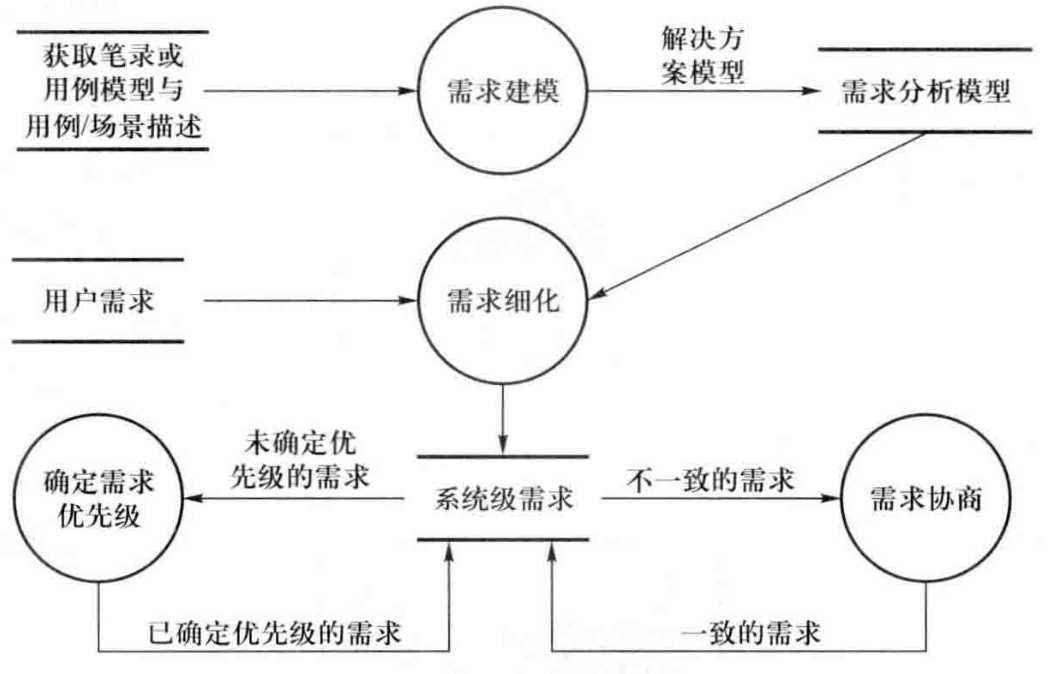
\includegraphics[width=0.65\textwidth]{img/后期需求阶段的需求分析活动流程图.png}
    \caption*{后期需求阶段的需求分析活动流程图}
    \vspace{-1em}
\end{figure}

\subsubsection{需求细化}
\begin{itemize}
    \item 明确用户需求的隐含因素 
    \item 将从问题域和业务的角度表述的用户需求等价的转化为从软件和技术的角度表述的系统需求 
    \item 非功能需求也需要从高层次的表述方式转化为一系列更加详细和具体的需求表述 
    \item 需求细化也会发现新的细节需求
    \item 需求已经得了充分的理解,并且开发者已经可以着手为其进行方案设计时停止细化过程 
    \item 细化后的需求应该被一一的标识和记录下来 
\end{itemize}

在分析活动当中需要收集每条需求的重要属性,常见的属性有以下几种
\vspace{-0.8em}
\begin{multicols}{2}
    \begin{itemize}
        \item 标识符,每一条需求都应该能够通过ID唯一的标识自己
        \item 源头,要能回溯到需求源头,例如特定的涉众
        \item 理由,需求被提出的目的
        \item 优先级,详细情况见下一节
        \item 成本,预估的实现成本
        \item 风险,实现该需求的过程中可能带来的风险
        \item 可变性,将来发生变化的可能性
    \end{itemize}
\end{multicols}

\subsubsection{确定需求优先级}
确定需求优先级的常用方法有下列几种:累计投票、区域划分、Top$-N$和数据量化

\textbf{累计投票:}在这种方法下,所有参与需求优先级评定的人员都会在一开始被给予一定数量的投票分数(如100分)。然后评定人员根据自己的判断将这些分数分配给各个单独的需求。最后,将每个需求得到的投票分值汇总,得到的总分值就代表了该需求的优先级,分值越大的需求优先级越高。

\textbf{区域划分:}在这种方法下,会将用来评价优先级的特征分为几个等级, 然后建立不同的优先级区域。最后,由评价人员将需求划分到不同的区域当中,每个区域的优先级等级就是该区域内所有需求的优先级。

\begin{table}[H]
    \centering
    \begin{tabular}{|c|c|c|}
    \hline
     & 重要 & 不重要 \\ \hline
    紧急 & 高优先级 & 不予处理 \\ \hline
    不紧急 & 中优先级 & 低优先级 \\ \hline
    \end{tabular}
    \vspace{-0.3em}
    \caption*{区域划分方法示例}
    \vspace{-1em}
\end{table}

可以用来评价优先级的常见特征有以下几方面
\vspace{-0.8em}
\begin{multicols}{2}
    \begin{itemize}
        \item 重要性。需求的不可或缺程度。
        \item 紧急性。需求的时间紧迫程度。
        \item 惩罚性。忽略需求会导致的惩罚程度。
        \item 成本。实现需求的代价。
        \item 风险。需求实现中可能产生的风险程度。 
    \end{itemize}
\end{multicols}
\vspace{-1em}

$\mathbf{Top}-\symbfit{N}$\textbf{:}这通常是在迭代式开发中使用的方法,如敏捷开发。在这种方法下,于每次迭代开始之前,由评价人选择他们认为最为重要的$N$个需求。这里$N$的取值是不受明确限制的,真正受限制的是Top $-N$个需求的实现代价总和。

\textbf{数据量化:}这种方法会将评价优先级的特征量化,然后再依据一定的计算规则计算需求最终的优先级。
\vspace{-0.3em}
$$\mbox{优先级}=\frac{\mbox{价值}\%}{(\mbox{成本\%}\times \mbox{成本权值}) + (\mbox{风险}\% \times \mbox{风险权值})}$$

\begin{figure}[H]
	\centering
    \vspace{-0.8em}
	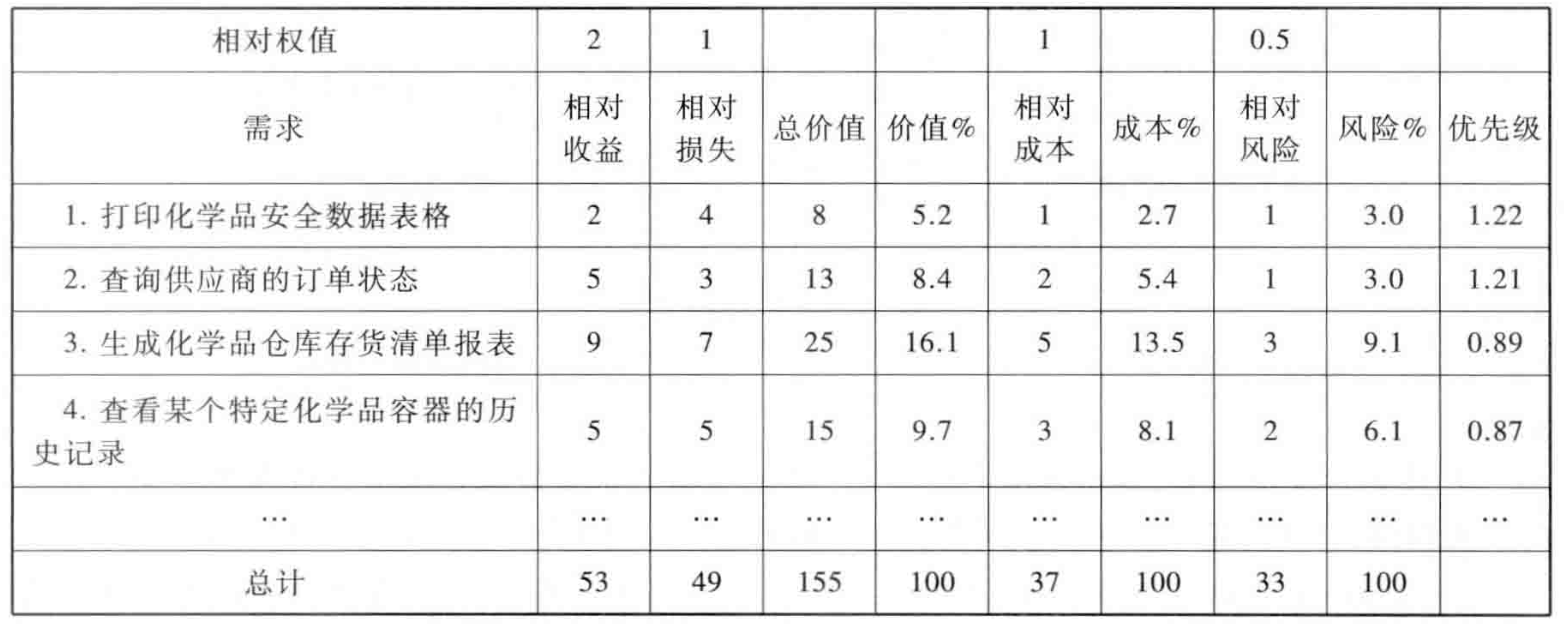
\includegraphics[width=0.85\textwidth]{img/QFD方法示例.png}
    \vspace{-1em}
\end{figure}

\vspace{-0.5em}
\begin{shaded}
    
\textbf{用户故事地图:}基于时间延迟成本的优先级判断
\begin{itemize}
    \item 延迟成本相同,短任务优先
    \item 工作量相同,高延迟成本优先
    \item 加权最短任务优先(重要$+$紧急程度)
    \item 所有优先级都是本地和临时的
\end{itemize}

\begin{figure}[H]
	\centering
    \vspace{-0.8em}
	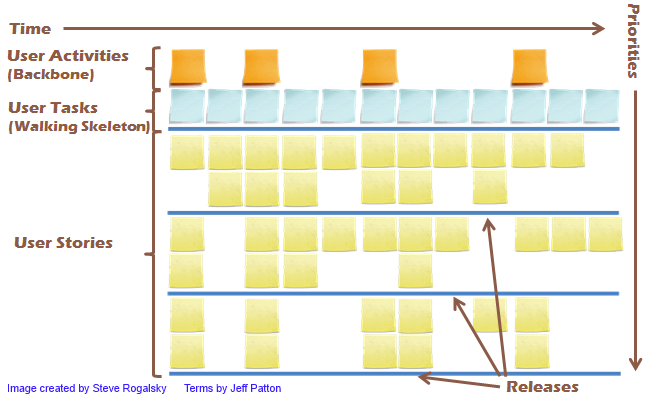
\includegraphics[width=0.6\textwidth]{img/用户故事地图.png}
    \vspace{-1em}
\end{figure}

\end{shaded}
\vspace{-1em}

\subsubsection{需求协商}
需求协商当中应该子以确保的3个原则
\vspace{-0.8em}
\begin{multicols}{2}
    \begin{itemize}
        \item 明确冲突的因素,避免情绪上的冲突
        \item 明确冲突的解决空间
        \item 确定最佳解决方案 
    \end{itemize}
\end{multicols}
\vspace{-1em}

\begin{figure}[H]
	\centering
    \vspace{-0.8em}
	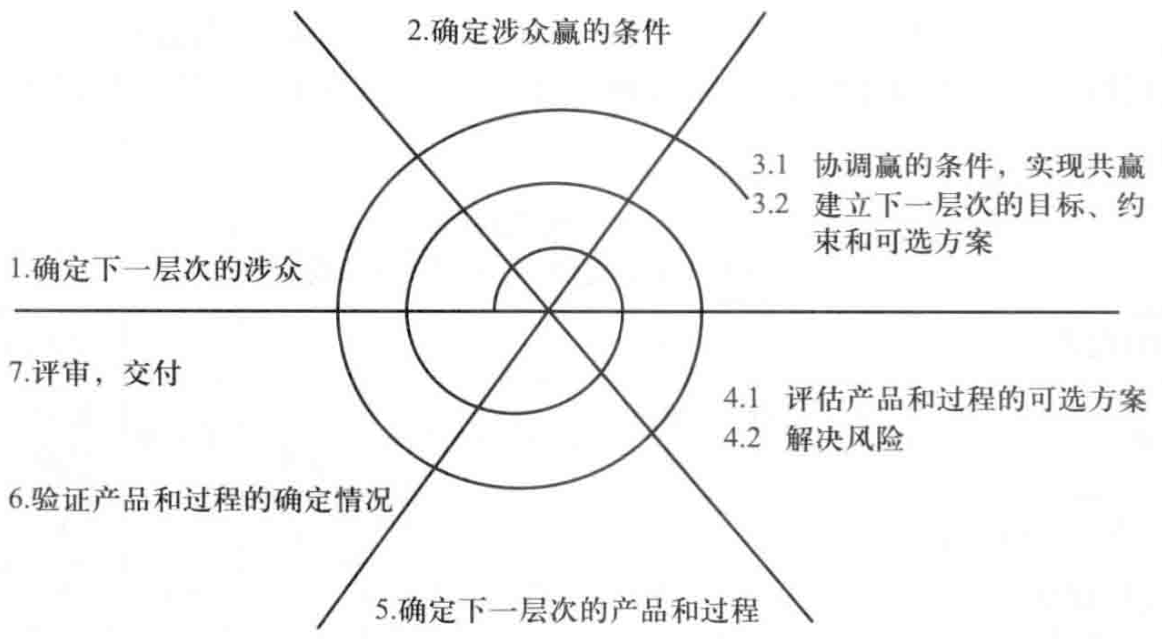
\includegraphics[width=0.67\textwidth]{img/WinWin螺旋模型.png}
    \caption*{WinWin螺旋模型}
    \vspace{-1em}
\end{figure}
